\chapter{Results: Spectroscopy}

The spectroscopy of Ba in SXe was studied in detail beyond that reported in \cite{Shon,Brian}, with the goal of imaging single Ba atoms.  Emission and excitation spectra are analyzed in \ref{sec:fluorescence}, with particular interest in the origin of the 619-nm peak in \ref{sec:619identification}.  Studies of temperature and bleaching effects in \ref{sec:tempanneal} and \ref{sec:bleaching} aid in determining optimal conditions for observation.  Backgrounds are analyzed in \ref{sec:bgs} in order to optimize sensitivity, and finally, candidate emission lines for Ba\textsuperscript{+} in SXe are discussed in \ref{sec:BaPlus}.

\section{Emission and Excitation of Ba in SXe}
\label{sec:fluorescence}

Deposits of Ba in SXe absorb primarily between 540~nm and 570~nm.  An absorption spectrum, obtained by observing absorption of white light by a large Ba deposit at 11~K, is shown in Fig. \ref{fig:BaAbs}, along with an example emission spectrum of a Ba\textsuperscript{+} deposit made at 45~K and observed at 11~K with 557~nm excitation.  Significant broadening, as well as a 4-nm redshift  of the central peak, occur relative to the vacuum $6s^{2}$ $^{1}$S$_{0} \rightarrow 6s6p$ $^{1}$P$_{1}$ absorption value of 553.5~nm.  Initial discovery of this absorption and emission was done with the purely neutral Ba getter source.  Observation of the same spectra from Ba\textsuperscript{+} ion beam deposits demonstrates some neutralization of the ions.  The fraction of ions neutralized is not determined.  \cite{Mong2015,Shon,Brian}

\begin{figure} %[H]
        \centering
                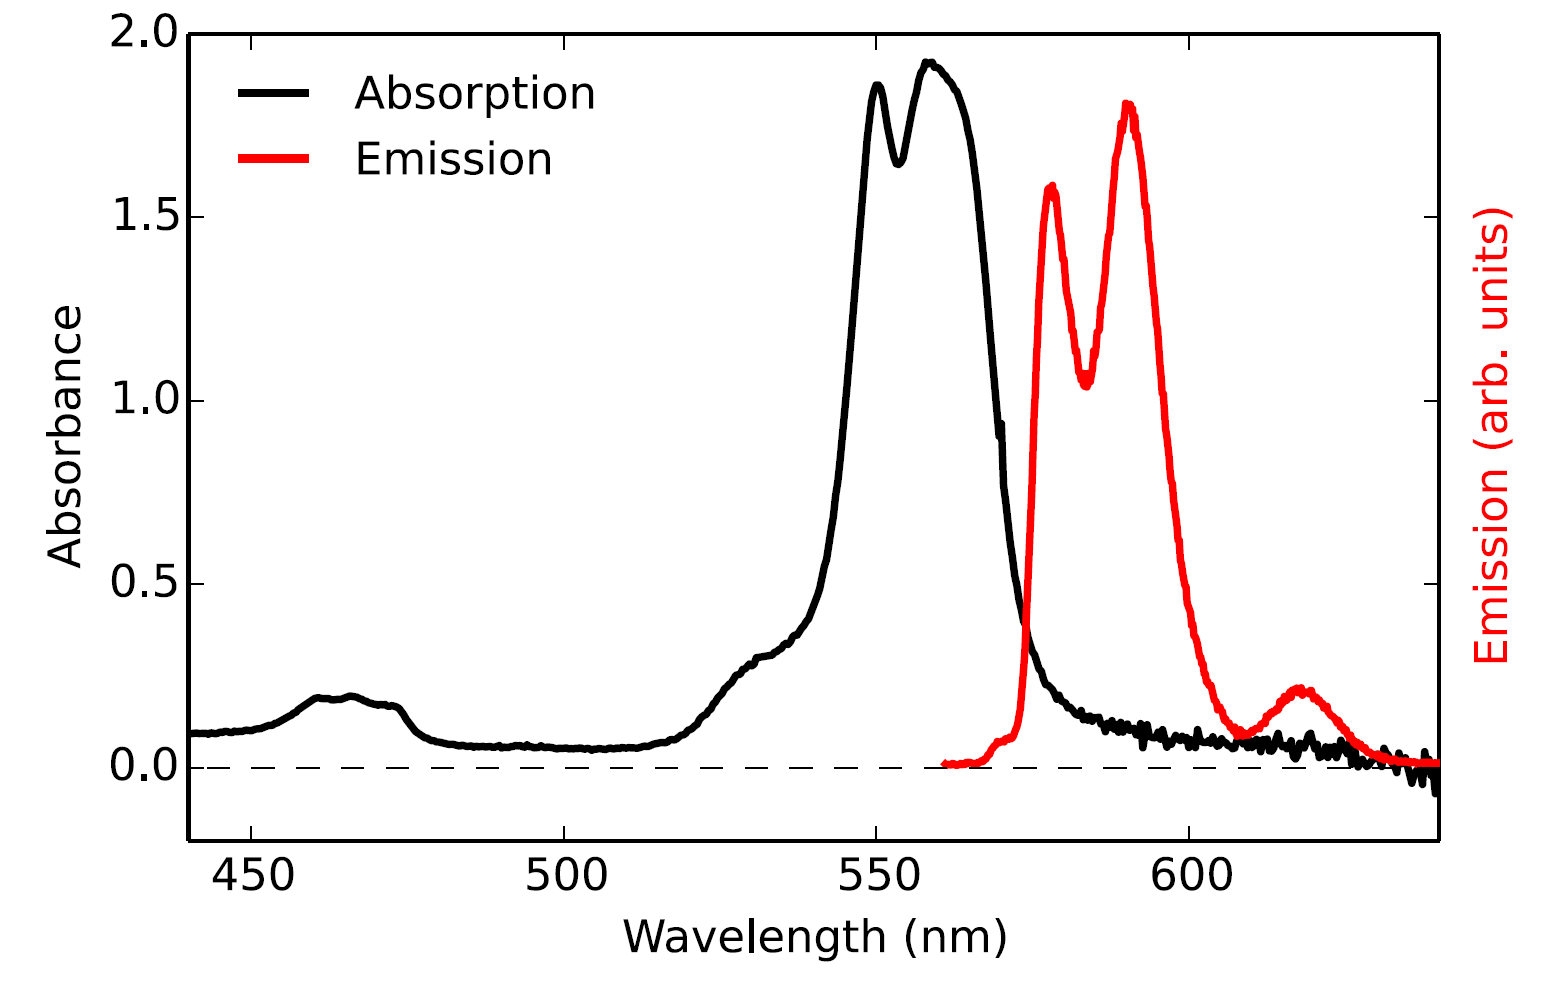
\includegraphics[width=.7\textwidth]{figures/BaAbs_fromBaSpec.png}
                \caption{Absorption and emission spectra of neutral Ba in SXe.  The absorption is of a Ba getter deposit at 10~K, and the emission is of a (neutralized) Ba\textsuperscript{+} deposit, deposited at 45~K and observed at 11~K with 557~nm excitation.\cite{Mong2015}}
\label{fig:BaAbs}
\end{figure}

\begin{figure} %[H]
        \centering
                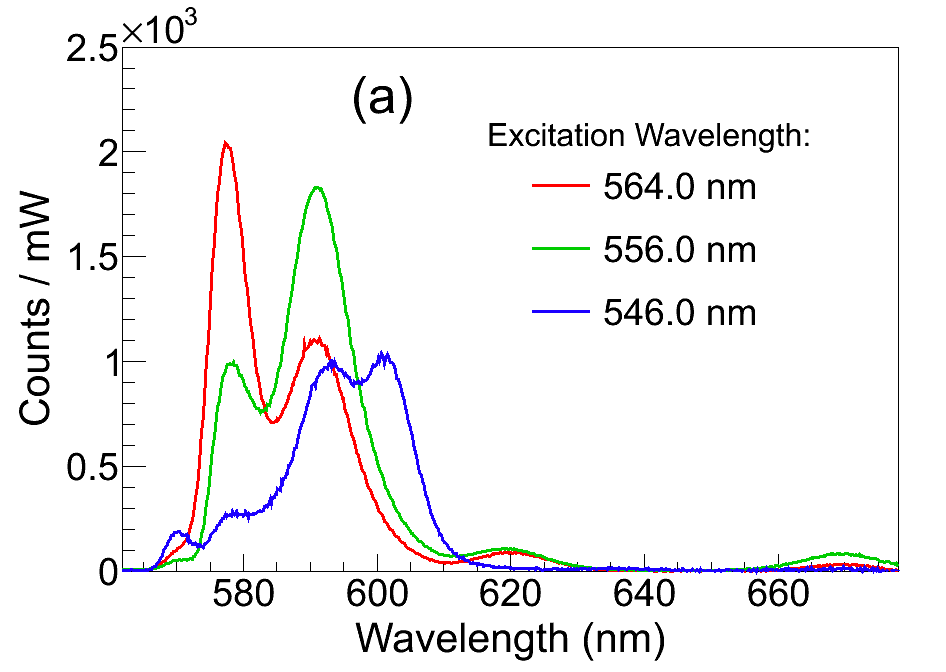
\includegraphics[width=.5\textwidth]{figures/excitspec_grn_spectra_v2.png}
                ~
                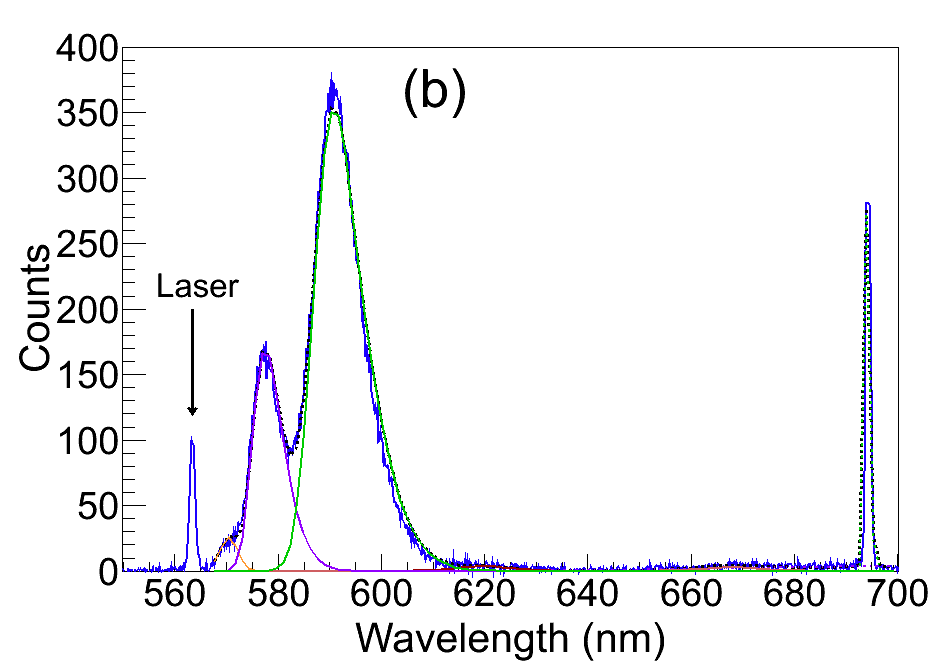
\includegraphics[width=.5\textwidth]{figures/excitspec_grn_spectra_fit.png}
                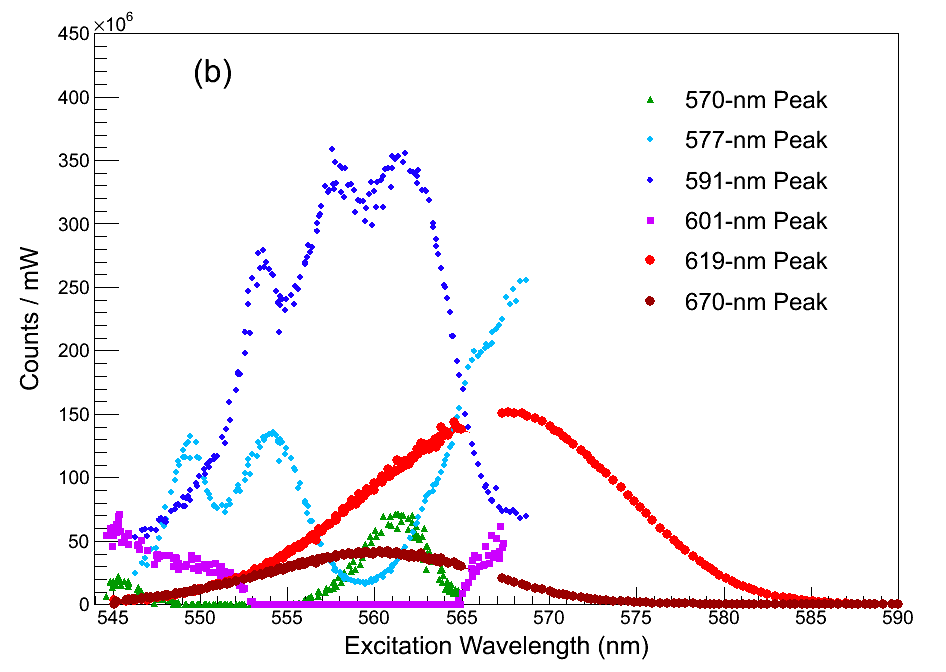
\includegraphics[width=.95\textwidth]{figures/excitspec_grn.png}
                \caption{Background-subtracted fluorescence spectra for a few different excitation wavelengths (a), an example fit to a spectrum (b), and full excitation spectra for all observed Ba fluorescence peaks (c).  Magnitudes in (c) have been scaled for visibility on the same plot (relative magnitudes are arbitrary as they are affected by relative site populations and fluorescence efficiencies).  The discontinuity around 566~nm for the 619- and 670-nm peaks is the boundary between usage of different laser dyes.  R6G dye is used for higher wavelengths and R110 for lower wavelengths and for all other curves.  Curves for the R6G segments (619- and 670-nm peaks) require special scaling to line up with their respective R110 segments, and this scaling was different between the 619- and 670-nm peaks, likely due to different relative populations of those sites on the different deposits.}
\label{fig:excitspecGrn}
\end{figure}

%Put legend in (b)? It's crowded.

%\begin{equation}
%A(1+erf(\frac{x-a}{\sigma_{1}})(1-erf(\frac{x-a}{\sigma_{2}}))
%\label{eqn:specfit}
%\end{equation}

The several red-shifted emission peaks observed are attributed to Ba atoms occupying different matrix sites in the SXe.  Deposition at temperatures higher than 11~K and exploration of more excitation wavelengths have led to discovery of a few emission peaks beyond the 591- and 577-nm peaks reported in \cite{Shon} and \cite{Brian}.  Emission spectra for selected excitation wavelengths are shown in Fig. \ref{fig:excitspecGrn}(a), for a deposit made at 44~K and observed at 11~K.  These selections are part of a full excitation spectrum, shown in Fig. \ref{fig:excitspecGrn}(c).  An excitation spectrum is produced by scanning the dye laser and measuring the magnitude of each fluorescence peak vs. excitation wavelength.  For each 1-s CCD exposure, a sum of \emph{\color{gray}don't call them this} asymmetric Gaussian functions and standard Gaussian functions is fit to the spectrum after pedestal subtraction.  The asymmetric Gaussian fit function used, which fits the 577- and 591-nm peaks somewhat better than standard Gaussians, is $A(1+$erf$(\frac{x-a}{\sigma_{1}})(1-$erf$(\frac{x-a}{\sigma_{2}}))$, where $A$ is the free amplitude parameter.  The peak position $a$ is fixed for each peak, as are the left and right smearing widths $\sigma_{1}$ and $\sigma_{2}$.  The function erf() is a Gaussian error function.  The asymmetric Gaussian function is not perfect for all frames, as the shape of the emission can depend on the excitation wavelength.  An example frame with fits is shown in Fig. \ref{fig:excitspecGrn}(b).  The full fit is the dotted black line, and each peak's contribution is in color.  Curves in (a) have about 100$\times$ the laser power used in the excitation spectrum (e.g. (b)) where low intensity is desired to avoid bleaching during the scan.  Rather than attempting frame-by-frame background subtractions, additional Gaussians are fit to the broad and sharp background fluorescence.  These backgrounds and their excitation spectra are discussed in \ref{sec:bgs}.  A 566~nm Raman filter was used to attenuate the majority of the laser scatter, however the small amount of scatter passed by the filter was used to determine the frame's excitation wavelength.  Each peak's fit contribution was then integrated and scaled by the frame's laser power, as the power output is not constant through the dye range.

%\emph{\color{gray}Care about 10~K excitation spectrum?}

Wavelength calibration was done using three lasers whose wavelengths were first measured with a Burleigh Wavemeter:  a red diode laser at 656.99~nm, a doubled Nd:YAG laser at 532.23~nm, and the C480 blue dye laser typically around 475~nm (at 488.91~nm for the data in Fig. \ref{fig:excitspecGrn}).  These lasers were directed at the same position on the sapphire window, and their scatter was imaged along the same path as the Ba fluorescence.  The WinSpec software applies the diffraction grating equation to calibrate each CCD pixel to a wavelength.

\section{619-nm Peak Identification}
\label{sec:619identification}

The 619-nm peak, as well as the 670-nm peak, was attributed to neutral Ba by a few further tests.  A large Ba\textsuperscript{+} deposit is compared to a deposit made with the Ba getter in Fig. \ref{fig:ArVsBa}(a).  The 619-nm and 670-nm peaks were observed with both sources, and since the getter produces only neutral Ba, they were attributed to neutralized ions in Ba\textsuperscript{+} deposits.  Observation of the fluorescence with two different types of Ba sources is itself positive.  In addition, observation of the fluorescence with the low deposit energy of the getter may bode well for the prospect of grabbing on a probe in LXe.  Observation of a large deposit of Ar\textsuperscript{+} in SXe is also shown in Fig. \ref{fig:ArVsBa}(a).  The lack of fluorescence further disfavors a matrix-damage-related source of the fluorescence, such as color centers.  Finally, to rule out the possibility that the signal in Ba imaging experiments is due to passed wavelengths far from the 620-nm band-pass region, e.g. infrared, imaging experiments of Ar\textsuperscript{+} deposits in SXe were performed with both pulsing and continuous ion beams.  The same 620-nm band-pass filter was used, as well as the same focused 570-nm laser, to be similar to Ba\textsuperscript{+} 619-nm imaging experiments.  Summed counts from these deposits were consistent with background, as shown in Fig. \ref{fig:ArVsBa}(b).

\begin{figure} %[H]
        \centering
                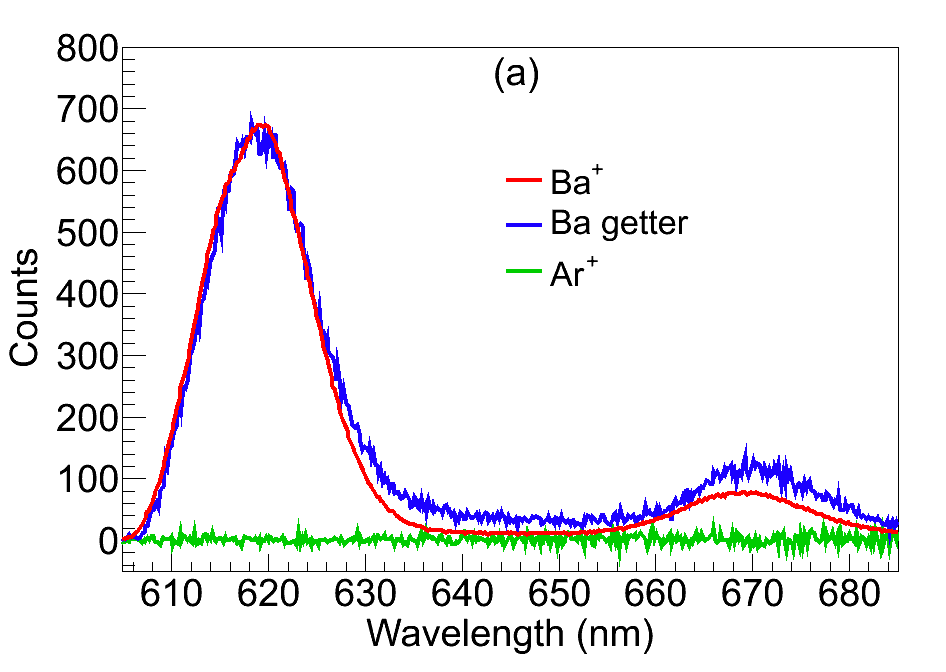
\includegraphics[width=.5\textwidth]{figures/Ar_vs_Ba.png}
                ~
                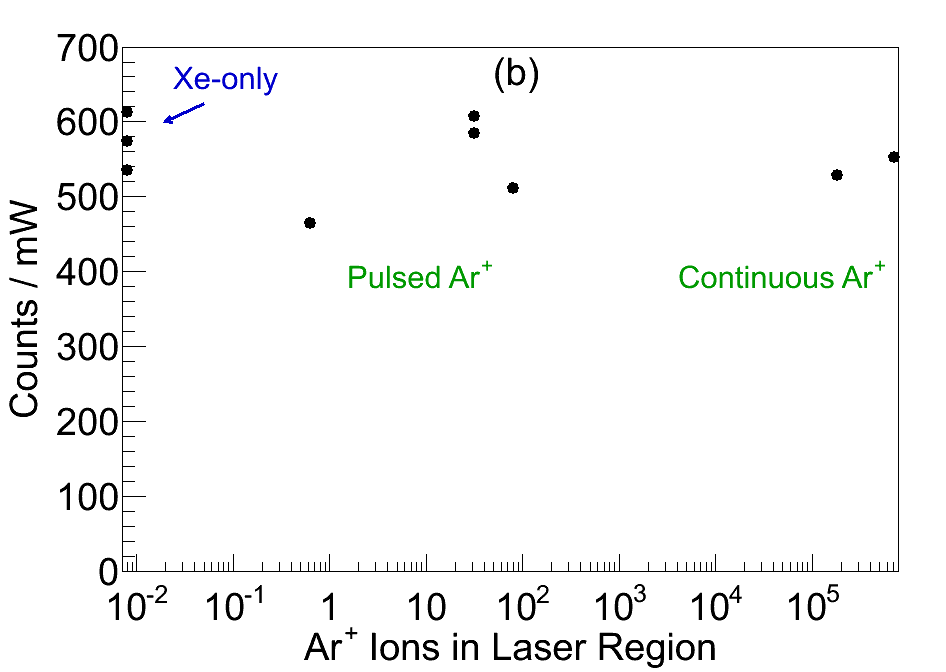
\includegraphics[width=.5\textwidth]{figures/ArImaging.png}
                \caption{Comparison of signal observed for deposits with the Ba\textsuperscript{+} ion beam (red), Ba getter (blue), and Ar\textsuperscript{+} ion beam (green) (a), and signal through 620-nm band-pass from deposits of small to large numbers of Ar\textsuperscript{+} ions in SXe.}
\label{fig:ArVsBa}
\end{figure}

%at one point youthought leak rate dependence could go here

\section{Annealing/Temperature Dependence}
\label{sec:tempanneal}

%\emph{\color{gray}When does it need to be mentioned that certain data was also used in the paper(s)?}

Matrix site occupancies for Ba atoms can depend on annealing history, and similarly on the temperature at which a deposit is made.  Spectra under different temperature conditions are shown in Fig. \ref{fig:specTempConditions}.  Peak shapes look similar for deposits made at 40-55~K as those made at 11~K and then annealed to 40-55~K, both being observed at 11~K, though relative amplitudes are not the same, likely due to matrix site populations.  Without annealing, 11-K deposits have a different peak shape around 590~nm, with a broader peak centered around 596~nm.  It is possible that the broader shape is due to a higher population of the 601-nm peak, and it is not resolved from the 591-nm peak.  The experiment in Fig. \ref{fig:specTempConditions} did not have optimal laser intensity for observing behavior of the 619-nm peak; a study of deposit conditions for this peak is shown in Fig. \ref{fig:specTempConditions619}.  In that experiment, the 619-nm fluorescence was observed in a focused laser beam at 570~nm, in an image through the 620-nm band-pass filter.  About 3$\times$ more 619-nm fluorescence was observed in the deposit at 52~K vs. 11~K for the same leak rate (the respective 31~nm/s and 37~nm/s are from the same Xe leak rate, resulting in different SXe deposition rates daccording to Fig. \ref{fig:fringes_52K_vs_11K}).  Also in this figure is a deposit at 11~K with the lower leak rate resulting in about 5~nm/s SXe deposition, which produced nearly 3$\times$ lower signal than the leak rate resulting in 37~nm/s SXe deposition.  Using the 10~K SXe density of 3.780~g/cm\textsuperscript{3} \cite{SXeDensity} and a typical Ba\textsuperscript{+} ion current density of 1.6~nA/mm\textsuperscript{2} at the sapphire window, 5~nm/s and 37~nm/s correspond to Xe:Ba ratios of about $8.7 \times 10^{3}$ and $6.4 \times 10^{4}$ respectively.  Xe leak rates above 37~nm/s result in rapid frosting of the SXe matrix, which causes blurring of the image and high laser scatter.  These tests guided the standard of depositing with Xe leak rate resulting in 31~nm/s SXe deposition at 50$\pm$5~K when observing the 577-, 591-, and/or 619-nm peaks.  The different bleaching behavior in the low Xe leak rate deposit is interesting but not well understood.

% is discussed briefly in \ref{sec:bleaching}.

%5.4E4 Xe:Ba for leak 48 50~K (31 nm/s)

\begin{figure} %[H]
        \centering
                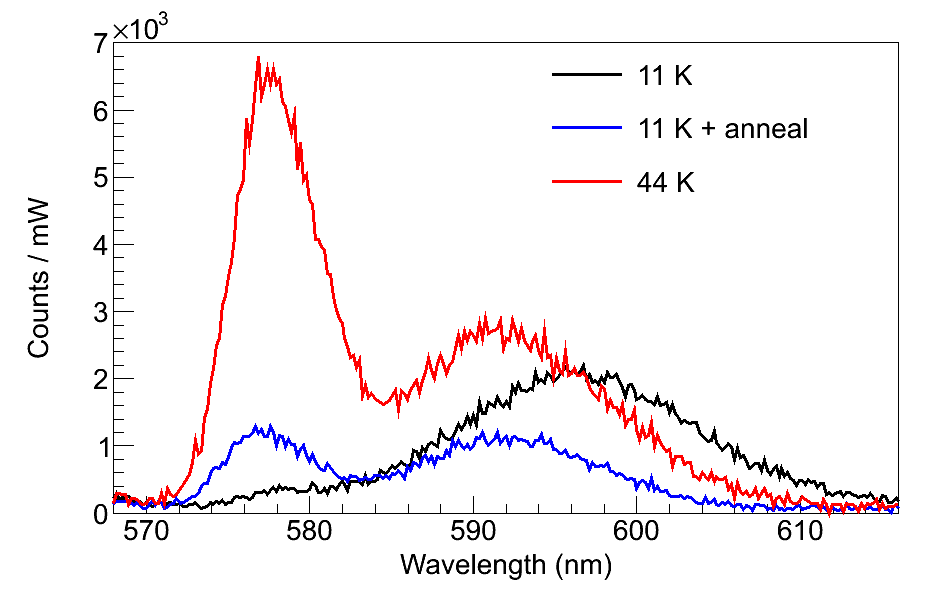
\includegraphics[width=.7\textwidth]{figures/spectra_temperature_conditions.png}
                \caption{Spectra of peaks around 590~nm of a Ba\textsuperscript{+} deposit made at 11~K before and after annealing to 39.4~K, and one made at 44~K.  All observations are at 11~K.  Both Ba\textsuperscript{+} deposits are 15~s, however the 44~K deposit is scaled slightly to account for different ion current.  Laser power was about 0.1~mW with an unfocused beam waist of w = 7.056~mm, at 566~nm wavelength.}
\label{fig:specTempConditions}
\end{figure}

\begin{figure} [h]
        \centering
                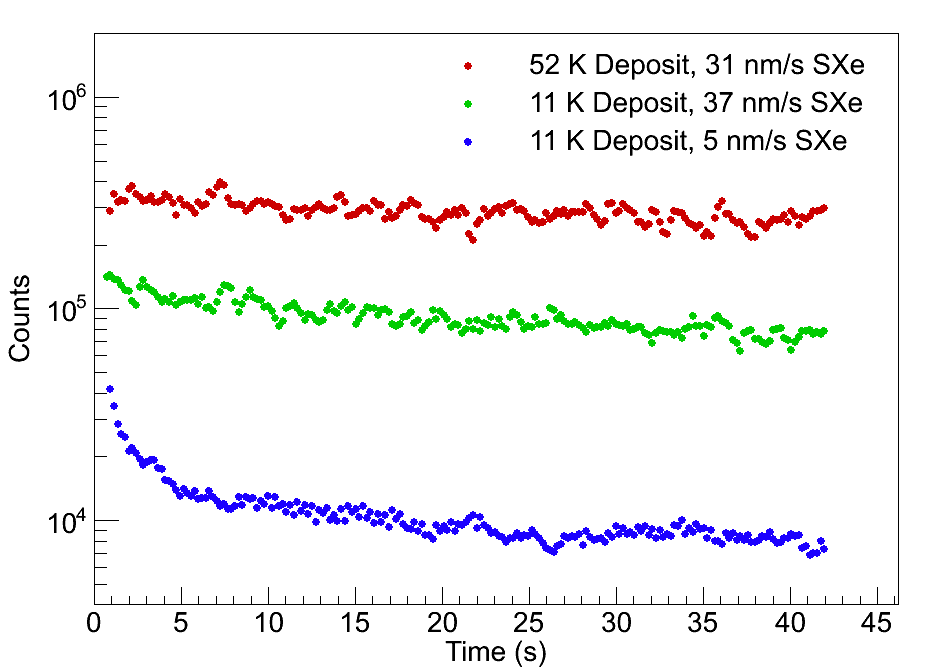
\includegraphics[width=.7\textwidth]{figures/619_deposit_conditions.png}
                \caption{619-nm fluorescence counts over time from imaging focused 570-nm laser region, for Ba\textsuperscript{+} deposits at different temperature and Xe leak conditions.  Frame times are 0.1~s, with time in between frames of about 0.11~s.}
\label{fig:specTempConditions619}
\end{figure}

\begin{figure} %[H]
        \centering
                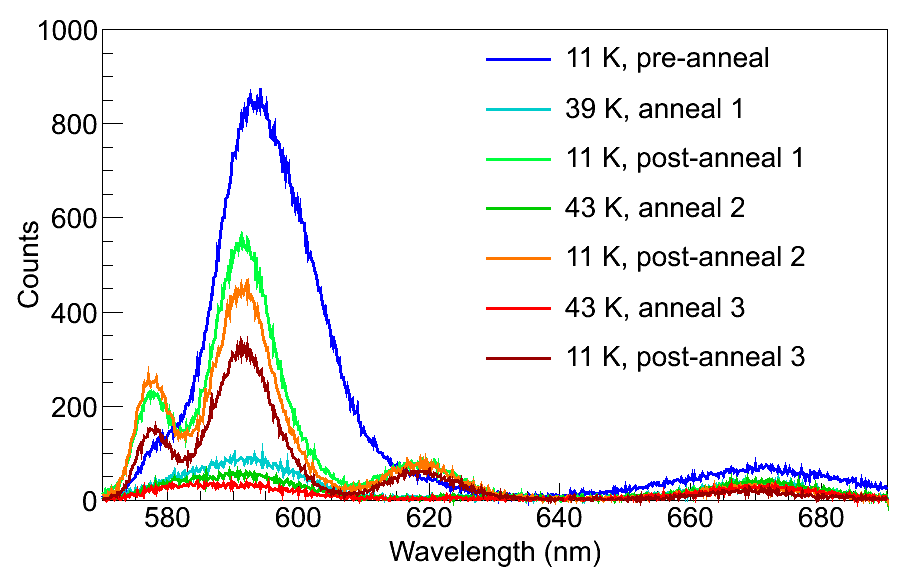
\includegraphics[width=.8\textwidth]{figures/spectra_annealing.png}
                \caption{Spectra of a large Ba\textsuperscript{+} deposit through several annealing cycles.  Initial deposit was at 11~K.  Laser power was about 0.2~mW with an unfocused beam waist of w = 7.056~mm, at 564~nm wavelength.  These are selections from the full data set shown as peak counts vs. temperature in Fig. \ref{fig:annealGrn}.  \cite{Mong2015}}
\label{fig:specAnneal}
\end{figure}

Fluorescence spectra with 564~nm excitation through several annealing cycles for a deposit made at 11~K are shown in Fig. \ref{fig:specAnneal}.  At this wavelength, all observed Ba peaks are prominent except the 570-nm peak.  Similar to excitation spectra, individual fluorescence peak amplitudes can be plotted vs. temperature by fitting the full spectrum in each frame.  Rather than asymmetric Gaussians, this analysis used standard Gaussian and Lorentzian functions.  Lorentzians fit the 619-nm and 670-nm peaks well.  Each individual peak's amplitude is plotted vs. temperature in Fig. \ref{fig:annealGrn}(b-f), with an example of a fit spectrum in Fig. \ref{fig:annealGrn}(a).  In this interpretation, the 601-nm peak along with the 591-nm peak fit the broader peak in the initial 11~K deposit.  The 601-nm peak had nearly complete loss in the first anneal cycle.  The 670-nm peak had significant loss, with more loss after each succeeding anneal cycle, each of which reached higher a temperature than the last.  The 591-nm had moderate loss with each cycle.  The 577-nm and 619-nm peaks gained significantly with the first anneal, suggesting that they are due to more stable matrix sites.  Both peaks remained about the same after the second cycle (small gain in 577-nm), and both had loss after the third cycle, which reached the higher temperature of 48~K. This could be due to greater diffusion at higher temperature leading to Ba/Ba interactions.

\begin{figure} %[H]
        \centering
                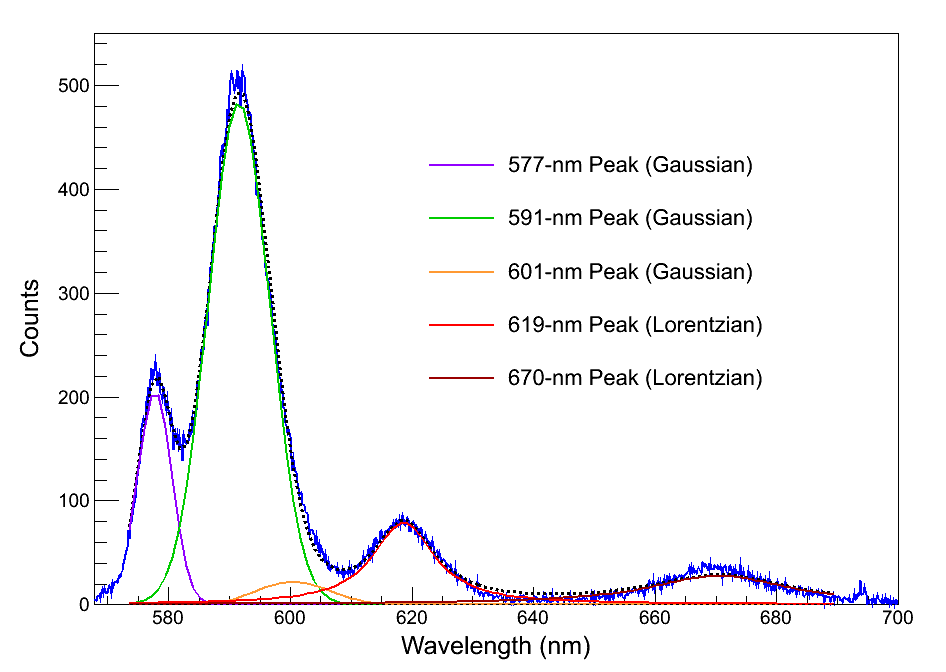
\includegraphics[width=.5\textwidth]{figures/spectra_anneal_fit.png}
                ~
                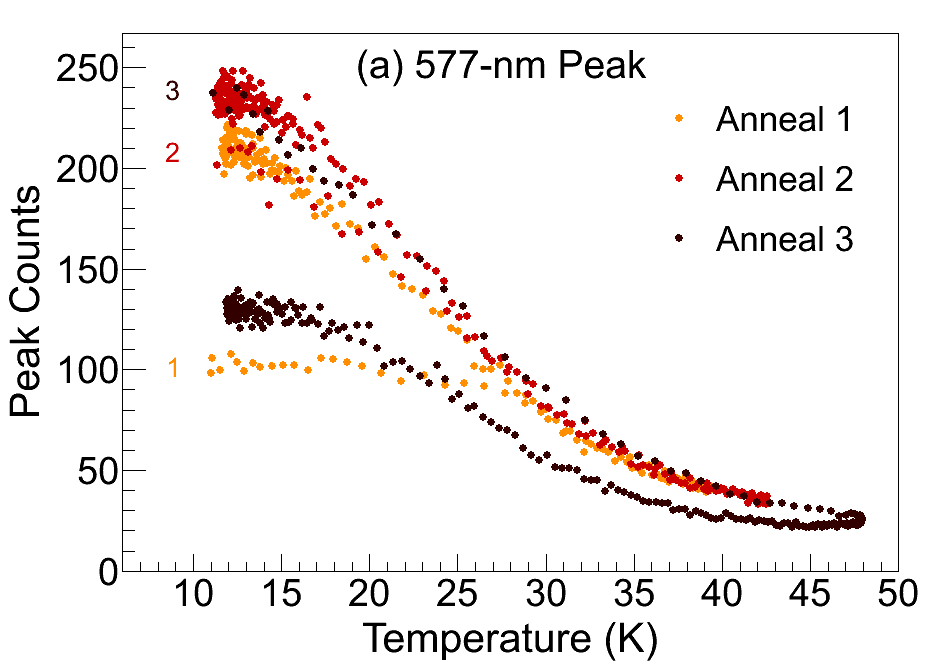
\includegraphics[width=.5\textwidth]{figures/anneal_577peak.png}
                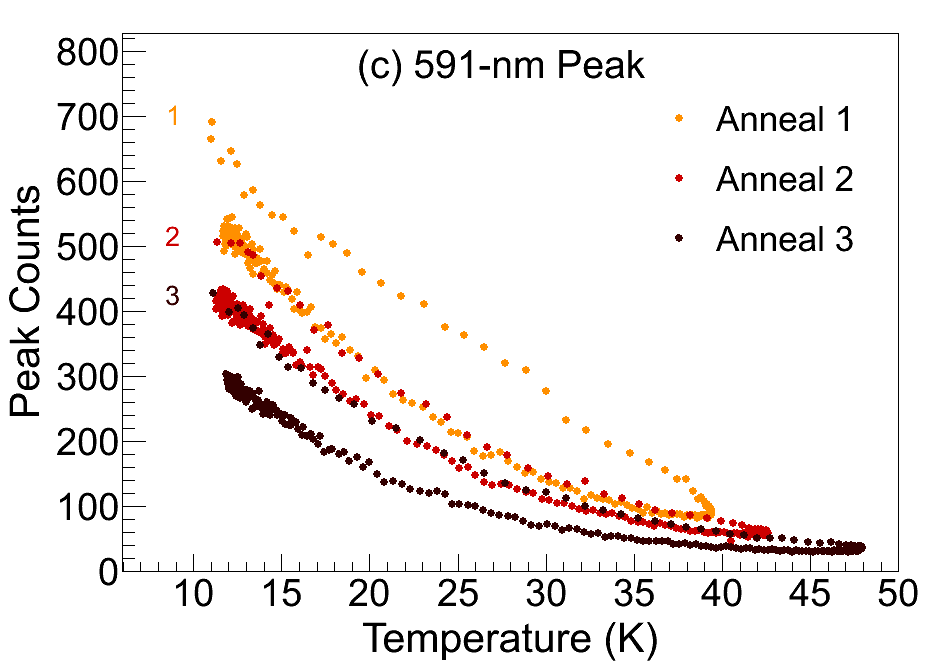
\includegraphics[width=.5\textwidth]{figures/anneal_591peak.png}
                ~
                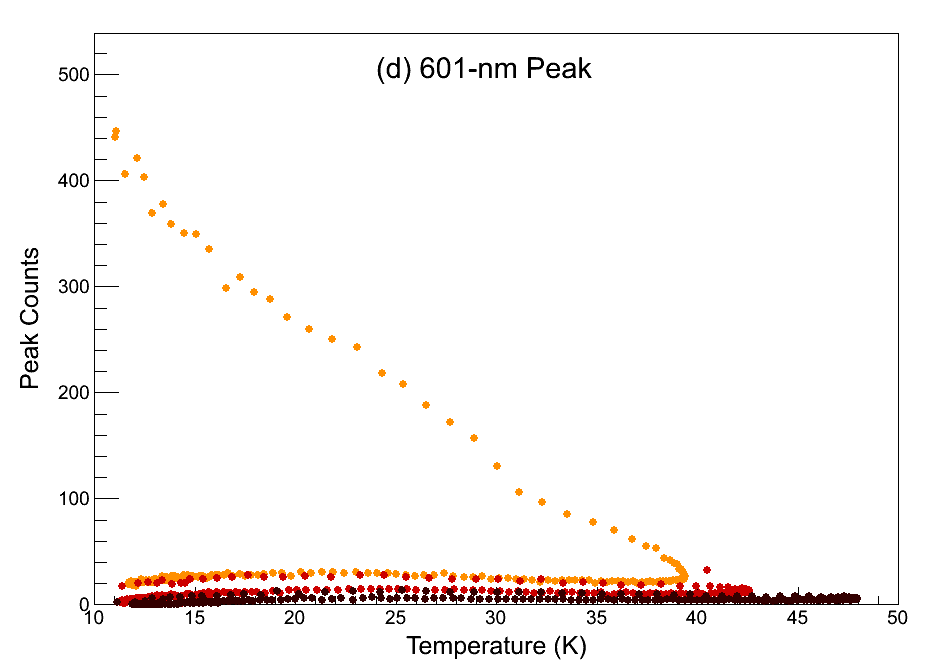
\includegraphics[width=.5\textwidth]{figures/anneal_601peak.png}
                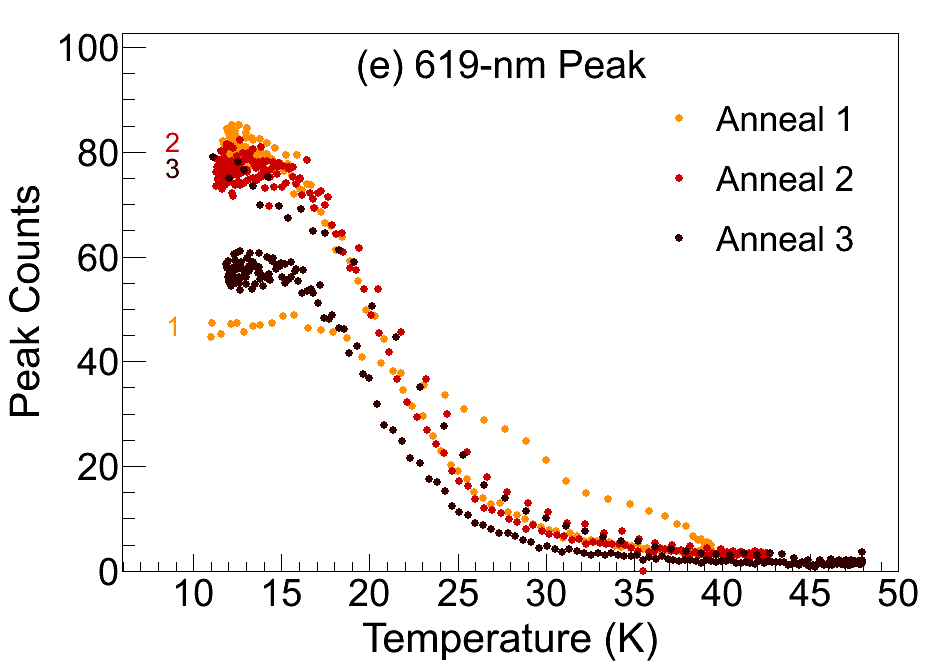
\includegraphics[width=.5\textwidth]{figures/anneal_619peak.png}
                ~
                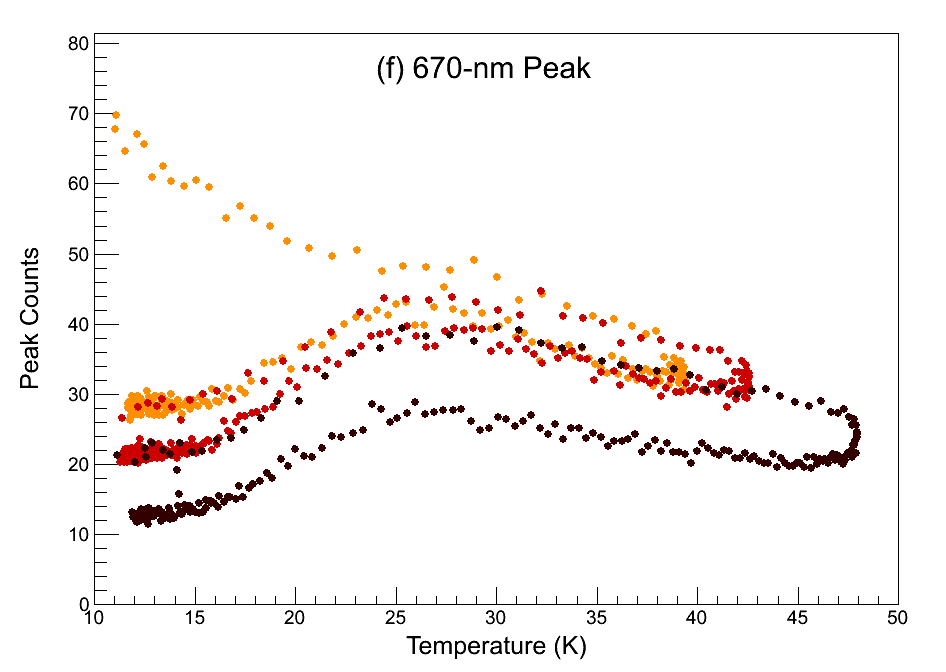
\includegraphics[width=.5\textwidth]{figures/anneal_670peak.png}
                \caption{Example fit with standard Gaussians and Lorentzians (a) and fit peak counts for each fluorescence peak through three annealing cycles of the Ba\textsuperscript{+} deposit made at 11~K (b-f).  ``1, 2, and 3" mark the beginning of each anneal cycle.  Laser power was about 0.2~mW with an unfocused beam waist of w = 7.056~mm, at 564~nm wavelength.}
\label{fig:annealGrn}
\end{figure}

Aside from matrix site changes, direct temperature dependence of fluorescence can be observed in annealing cycles.  The 577-, 591- and 619-nm peaks have their highest amplitude at 11~K.  The 577-nm and 619-nm peaks appear to be leveled off at 11~K, while the 591-nm may benefit from even lower temperatures.  The 670-nm peak has its highest amplitude at around 25~K (apparent after its major site alteration has occurred).  This inverse relationship between fluorescence and temperature suggests that a probe in nEXO will need to be moved to an evacuated chamber in order to cool to 11~K or below for observation.  

%\emph{\color{gray}601 and (not shown) 570 would require different wavelength to study.}

%[inverse relationship] could be due to a different matrix environment at higher temperature, or possibly a loss of fluorescence efficiency due to increased non-radiative decays from the excited state.  

\section{Bleaching}
\label{sec:bleaching}

\emph{\color{gray}Just show bleaching, as informant on how to image, rather than showing model fits.}

Decay of fluorescence with laser exposure, or bleaching, was observed for all six Ba fluorescence peaks.  It is a rapid process for the 570-, 577-, 591-, and 601-nm peaks, and a much slower process for the 619- and 670-nm peaks.  With the prospect of counteracting the effect for single-atom imaging, bleaching of the 577- and 591-nm peaks was studied in detail by observing the fluorescence decay rate for varying excitation rates.  

\begin{figure} %[H]
        \centering
                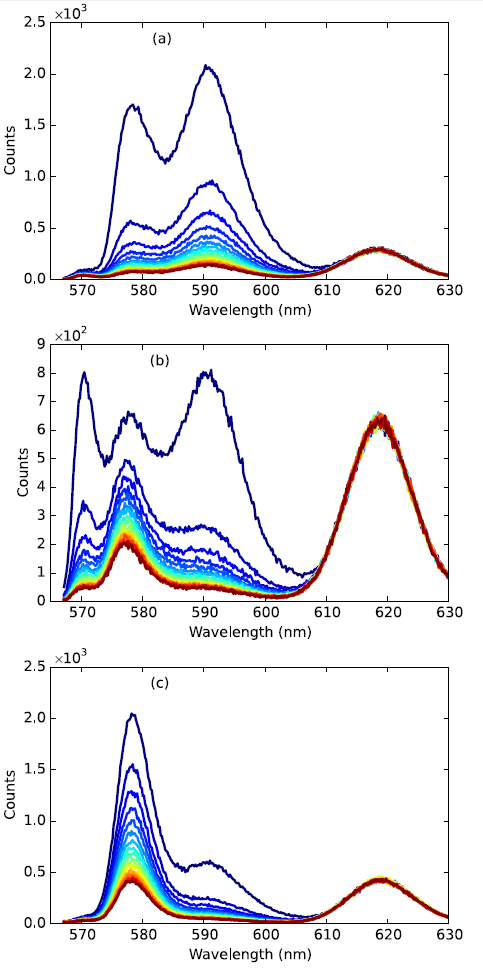
\includegraphics[width=.5\textwidth]{figures/bleach_spec.png}
                \caption{\color{red}will re-do these, ideally showing 670-nm. \cite{Mong2015}}
\label{fig:specBleach}
\end{figure}

To produce a well-known laser intensity, the laser was de-focused to a specific beam waist (w), and the image of 619-nm fluorescence (which defines the laser region due to its low bleaching) from a large Ba\textsuperscript{+} deposit was centered in the spectrometer slit and a y-pixel region of interest (ROI) with edges at 90\% of the maximal intensity.  Ba spectra over time are shown in Fig. \ref{fig:specBleach}(a,b,c) for excitation at (a) 556.9~nm, (b) 562.6~nm, and (c) 566.3~nm, where relative bleaching rates between peaks can be seen to depend on the excitation wavelength.  Fluorescence counts vs. total excitations (excitation rate $w_{12}$ $\times$ time) for the 570-, 577-, and 591-nm peaks are plotted in Fig. [fig bleaching].  \emph{\color{gray}...I swear this doesn't make sense, because you KNOW 1/x$\times$t and x$\times$I does not yield the same total counts...\textbf{maybe you just want to globalize ones with the same I and t, or just compare differently}} \emph{\color{red}don't forget the correction on p-meter sensitive area and on p-meter quantum efficiency}  Note that the 577-nm peak has a lower bleaching rate when excited in the region around {\color{red}566}~nm.  This informed the usage of {\color{red}x}~nm in imaging this fluorescence in \ref{sec:imaging590and577}.

The 6-level model solved in [sec. in Ch. 2] can be applied to this bleaching data to determine deviations from vacuum transition rates.  The 6\textsuperscript{th} level allows for one additional vacuum-forbidden transition from the excited state, $a_{26}$ and its decay back to ground $a_{61}$, e.g. a \textsuperscript{3}P state.  A successful model will fit observed bleaching curves for all values of $w_{12}$ with the same transition lifetimes.  An example \emph{\color{gray}examples of} of a good model fit\emph{\color{gray}s} is shown in Fig. \ref{fig:bleachModel}.   The nearly constant decay slope in later frames was easily fit with the introduction of non-zero $a_{26}$, and could not be fit by manipulation of the existing transitions, suggesting the presence of an additional matrix-induced path out of the excited state. In addition, non-zero $a_{61}$ values only hurt the fit, suggesting that this state does not have a spontaneous recovery path  \emph{\color{gray}(is this just for one of the peaks?)}.  An important observation is that the other rates do not require much change from their respective vacuum values, with the exception of \emph{\color{gray}whatever that one is.}  \emph{try non-changed $a_{2?}$, to see if maybe the extra .5-s is actually in between each frame ... \textbf{go into the lab and try come where this ,5-s would dominate and see if it's there}}  This suggests that the observed bleaching is mostly due to optical pumping into the metastable D states, with the exception of $a_{26}$, and thus that laser re-pumping should be possible to increase the fluorescence signal from these peaks.

\begin{figure} %[H]
        \centering
                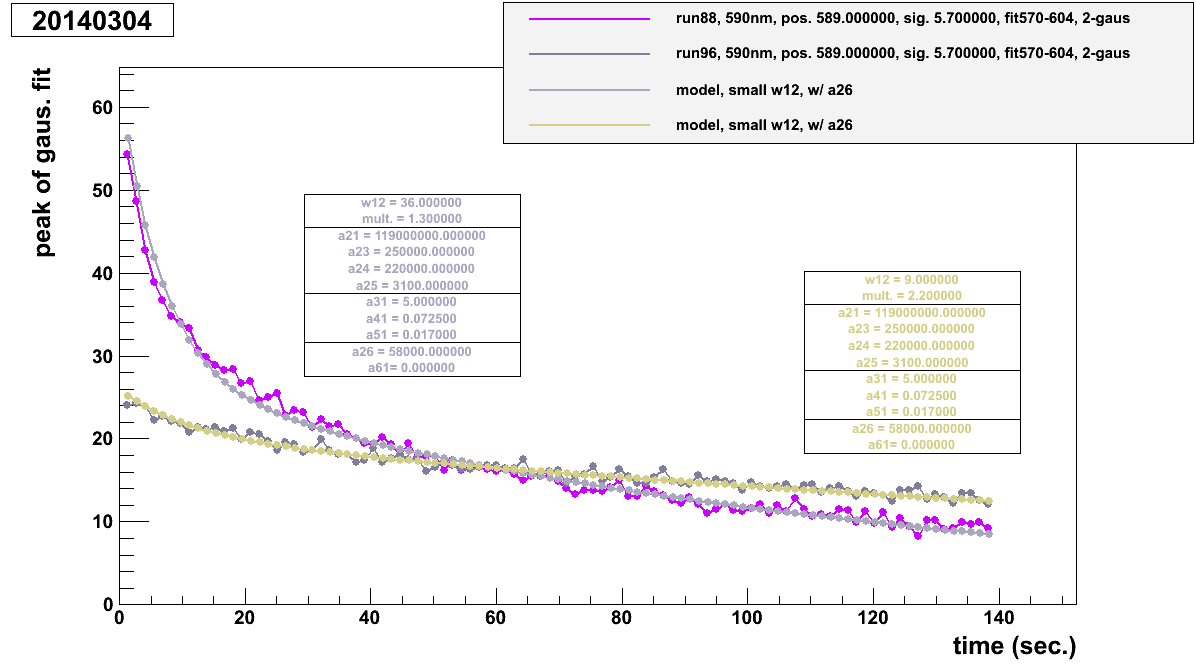
\includegraphics[width=.7\textwidth]{figures/model_smallw12_a26_run96and88_close.png}
                \caption{\color{red}example place-holder}
\label{fig:bleachModel}
\end{figure}

Another interesting result is the model's inability to explain the low fluorescence efficiency ($\epsilon_{f}$) observed in these peaks.  The number of counts observed is significantly lower than expected from $a_{21} = ?$.  $\epsilon_{f}$, defined in [Ch.2], was measured by the total counts observed in the first frame of exposure divided by its respective $w_{12}$, shown in Fig. \ref{fig:qe}.  This method of measuring $\epsilon_{f}$ becomes less accurate with more optical pumping in the first frame, i.e. with higher $w_{12}$ for a given frame time.  Thus, the trend should be extrapolated toward zero.  Since it seems to be leveling off in the lowest $w_{12}$ values,  the trend suggests a real $\epsilon_{f}$ of about {\color{red}0.5\%}.  The bleaching model was unable to explain this low $\epsilon_{f}$ by additional paths out of the excited state without introducing extreme alterations to existing rates, or by introducing extreme $a_{26}$ and $a_{61}$, in order to dominate $a_{21}$.  A possibility is that the low count rate actually reflects a matrix site population by only about 1\% of deposited Ba\textsuperscript{+} ions.  \emph{\color{gray}I bet $w = 100~\mu m$ is more likely to be the wrong one ... does that one require that more extreme w12 change in modeling (or, the one that still requires a fix after the right P correction has been applied)?}

\begin{figure} %[H]
        \centering
                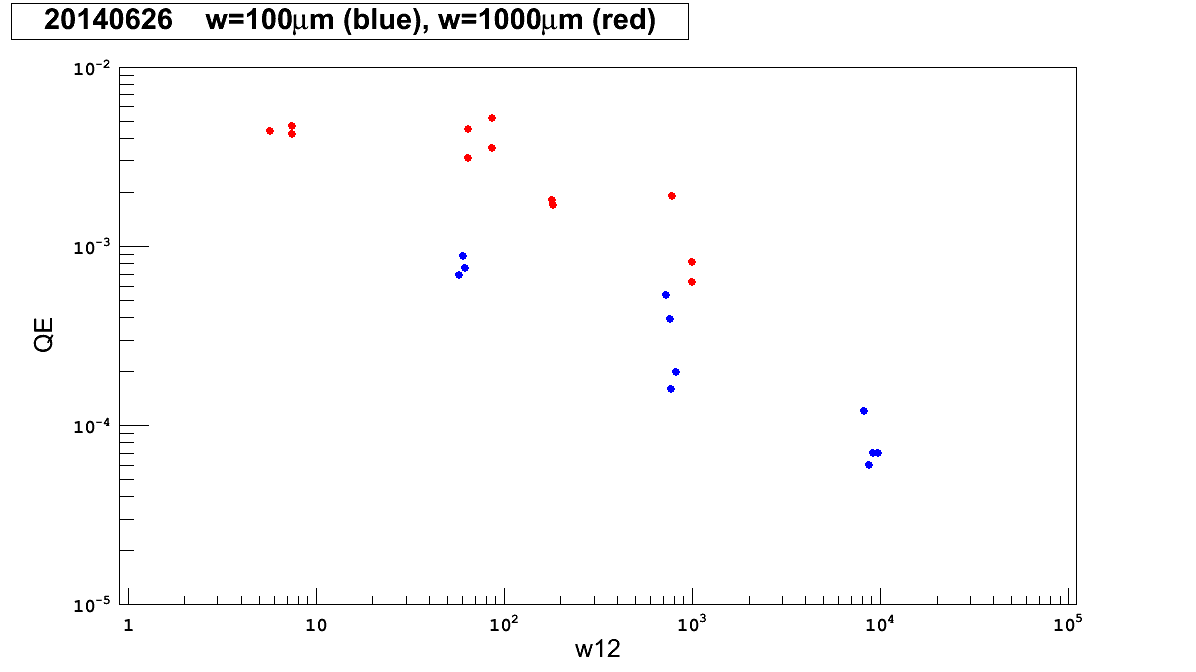
\includegraphics[width=.7\textwidth]{figures/QE_20140626_separate_w.png}
                \caption{\emph{\color{gray}correct this too for real w12}, and needs some correction to combine the two regions?}
\label{fig:qe}
\end{figure}

%\begin{figure} %[H]
 %       \centering
  %              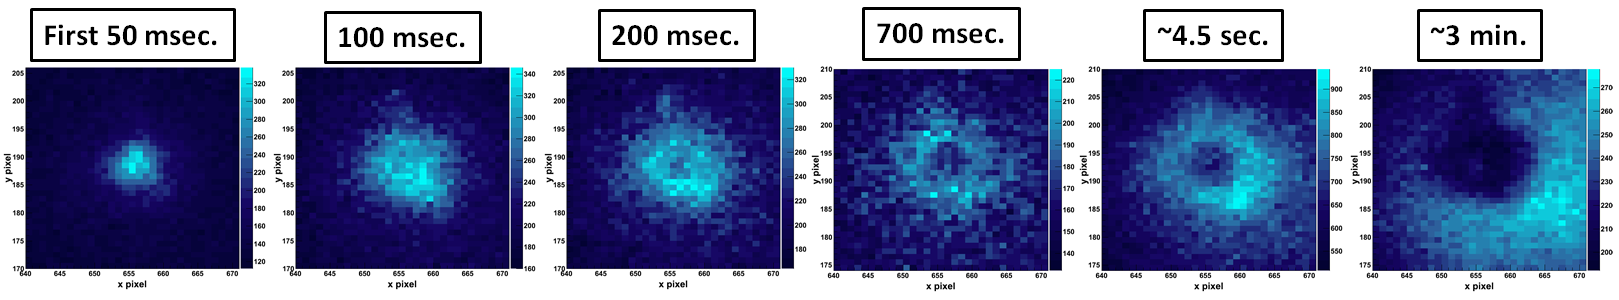
\includegraphics[width=.9\textwidth]{figures/hole_bleach_590.png}
   %             \caption{}
%\label{fig:testfig}
%\end{figure}

Effective re-pumping of optically pumped Ba could require up to three additional lasers, one for each of the populated metastable D states, as it does in vacuum.  The optimal absorption for each transition would need to be discovered using tunable lasers in the infrared, and the search would be challenging, as the effect of re-pump is small until all three are achieved.  However, mixing of states in the Xe matrix could lower the number of lasers needed.  Searches for an effect of additional excitation lasers were attempted with a few different lasers.  A 1550-nm diode laser and a 1064-nm Nd:YAG laser were used to attempt re-pumping from the \textsuperscript{1}D and \textsuperscript{3}D states, respectively.  A 657-nm diode laser was used to attempt excitation from the \textsuperscript{3}D states into the higher-level $5d6p$ \textsuperscript{3}D$_{1}$\textsuperscript{o} state, which in vacuum has a path back to ground, as utilized in the Ba MOT in \cite{BaMOT} for the $6d5d$ \textsuperscript{3}D$_{1}$ state with 659.7~nm.  The blue C480 dye laser and 406-nm Kr ion laser were used to attempt excitation from the \textsuperscript{1}D state into the higher-level states $6s7p$ \textsuperscript{1}P$_{1}$\textsuperscript{o} and $6s8p$ \textsuperscript{1}P$_{1}$\textsuperscript{o}, respectively, which have paths back to ground in vacuum.

The only effects observed on bleaching rates by these re-pump lasers were increased bleaching by the blue dye and 406-nm Kr ion lasers.  Some effect of a return of fluorescence was observed after separate exposures of low-intensity 406-nm Kr ion laser, shown in Fig. [fig Kr return].  In this experiment, bleaching of the 591-nm peak was observed by x-nm excitation, and then the x-nm laser was blocked for a length of time, either for a waiting period or for exposure to the 406-nm laser.  Larger returns in 591-nm fluorescence were observed with 406-nm exposure than for periods of just waiting, for low intensities of the 406~nm.  However, co-exposure of this intensity of 406~nm with the green excitation laser had no noticeable effect.  This phenomenon was not explored further.

%Another possible mechanism for bleaching is matrix site change caused by the difference in the Ba-Xe interactions when the Ba is in the excited state.  This was explored in an experiment where excitation spectra were produced before and after bleaching the Ba sample at various wavelengths.  \emph{\color{gray}Selected} runs are shown in Fig. [bleaching excitspec].  \emph{\color{gray}describe -- interesting changes may reveal different site components of the peaks -- or does it?  idk how this could happen ... cuz the triple peak thing was supposedly normal for a single site ... small rises were ween, but poplulations cannot be known, so we don;t know}  \emph{\color{red}plots could be simple, like 2 excitspec for a single peak with an arrow at the bleaching (between) $\lambda$ w/ a note like ``bleach w/ x~mW of x~nm"...}

The 619-nm peak bleaches at much higher laser intensities.  At a few mW of around 570~nm, bleaching is observed when the laser is focused.  Integrated 619-nm fluorescence, divided by laser power, vs. time from an image of a focused 570-nm laser is shown in Fig. \ref{fig:bleaching619} for three laser powers.  Observation of lower total counts when laser intensity and exposure time are increased and decreased, respectively, by the same factor, i.e. the same number of photons on faster time scales, indicates a time-dependent return mechanism for the fluorescence.  This could be a return from a metastable state.  Alternatively, if the 619-nm bleaching is caused by laser-heating of the sample (likely by heating the sapphire window), then the time-dependent return could be defined by the cryostat cooling power.  Faster exposure times are more convenient, however this must be balanced against a loss of signal-to-noise.  The 0.21~mW laser power was chosen, corresponding to an intensity of about 11.8~$\mu$W/$\mu$m$^{2}$.

\begin{figure} %[h]
        \centering
                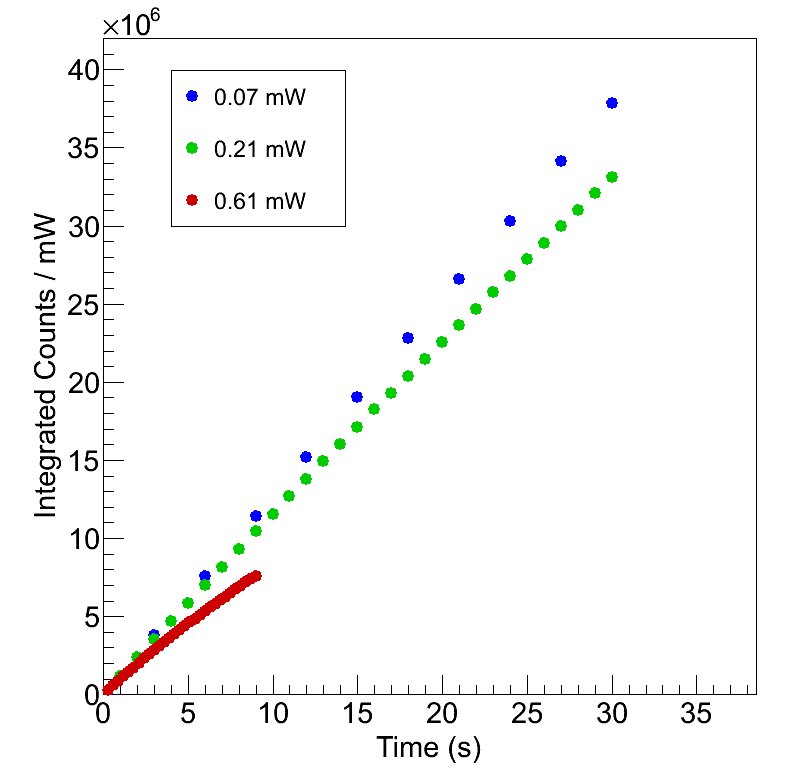
\includegraphics[width=.7\textwidth]{figures/619_bleach_summed_per_mW.png}
                \caption{}
\label{fig:bleaching619}
\end{figure}

%As indicated in Fig. \ref{fig:specTempConditions619} in \ref{sec:tempanneal}, more rapid bleaching of the 619-nm peak is observed with the lower SXe growth rate of 5~nm/s.  This is not understood, though possible explanations include 

\section{Backgrounds}
\label{sec:bgs}

\emph{\color{gray}Should \textbf{show} the S/sqrt(B), and perhaps do a new one with the surf-bg-dominated spectrum to say maybe x should be used instead, but maybe not.}

One source of background emission was observed from the surfaces of the window.  Its broad fluorescence is shown in Fig. \ref{fig:surfBG}(a) with a 610-nm Raman filter cutoff and 570.4~nm excitation, and its excitation spectrum is shown in Fig. \ref{fig:surfBG}(b) over the R6G dye range.  The nature of this emission has not been determined, however a few features were identified.  One was that the emission increased as the window temperature was decreased, down to about 100~K where it remained flat down to 11~K, shown in Fig. \ref{fig:BGtempDependence}.  Another feature of the surface background is that it bleaches with laser exposure.  This was useful in that the background could be reduced by pre-bleaching of the window.  However, the bleaching behavior also presented an inconvenient time dependence of the surface background, as historical bleaching and possible slight movements of the laser could lead to variation.  Frequent Xe-only deposits were made in order to establish proper background subtraction.  Spacial variation in the background is especially cumbersome in a laser scanning experiment, as discussed in \ref{sec:scanning}.  Given these behaviors, it is possible that the surface background is caused by a species which freezes to the window, or something which coats the window and fluoresces more at lower temperatures.  In either case, the bleaching could be explained by evaporation with laser heating, or by optical pumping of the species into a metastable state.

%, shown in Fig. [fig surfaceBG bleaching]

\begin{figure} %[H]
        \centering
                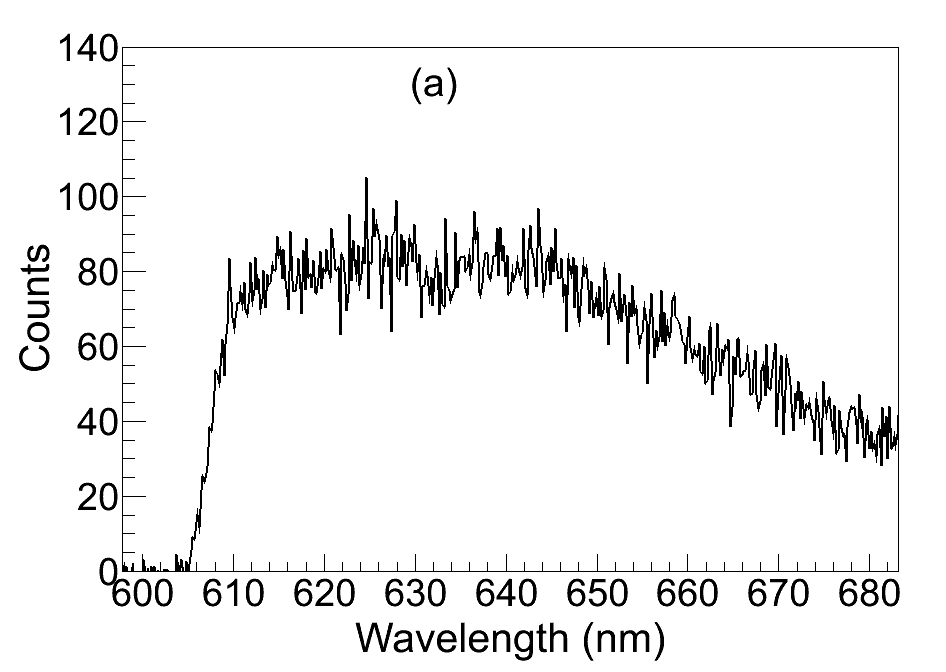
\includegraphics[width=.7\textwidth]{figures/surfaceBG_a.png}
                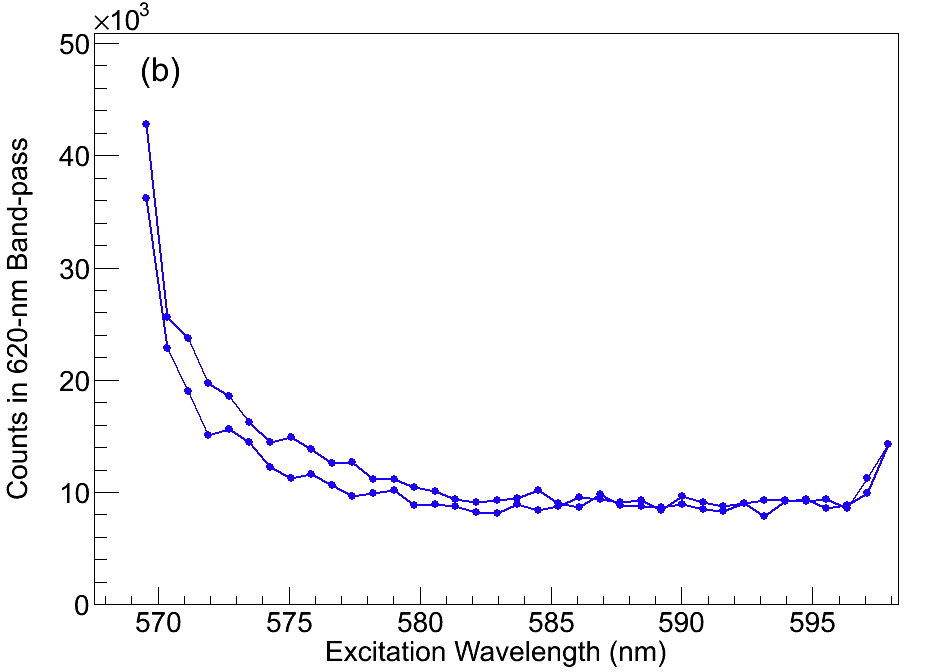
\includegraphics[width=.7\textwidth]{figures/surfaceBG_b.png}
                \caption{Surface background emission spectrum w/ excitation at 570.5~nm (a) and its excitation spectrum in R6G dye range (b).  The sharp drop in (a) around 608~nm is the Raman filter cutoff.}
\label{fig:surfBG}
\end{figure}

\begin{figure} %[H]
        \centering
                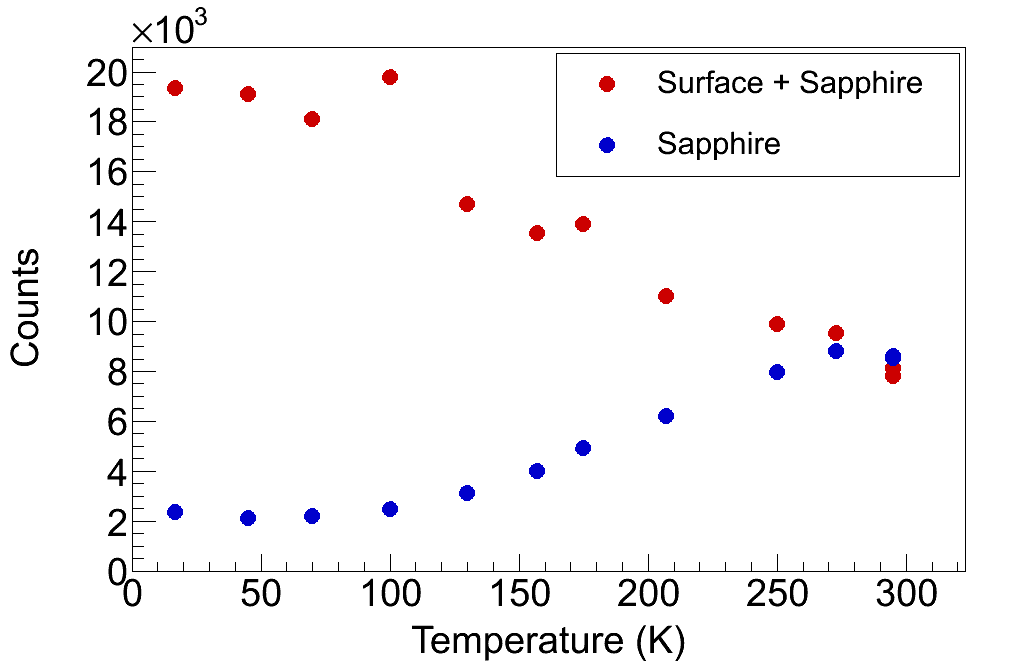
\includegraphics[width=.6\textwidth]{figures/bg_temp_dep.png}
                \caption{Temperature dependence of surface (red) and sapphire bulk (b) backgrounds.}
\label{fig:BGtempDependence}
\end{figure}

\begin{figure} %[H]
        \centering
                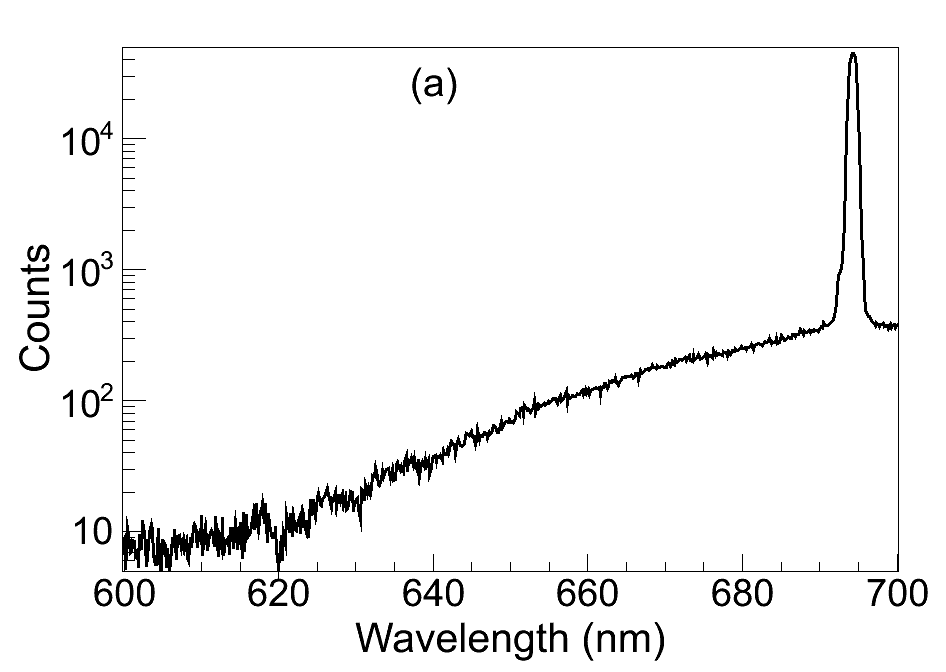
\includegraphics[width=.7\textwidth]{figures/Cr_a.png}
                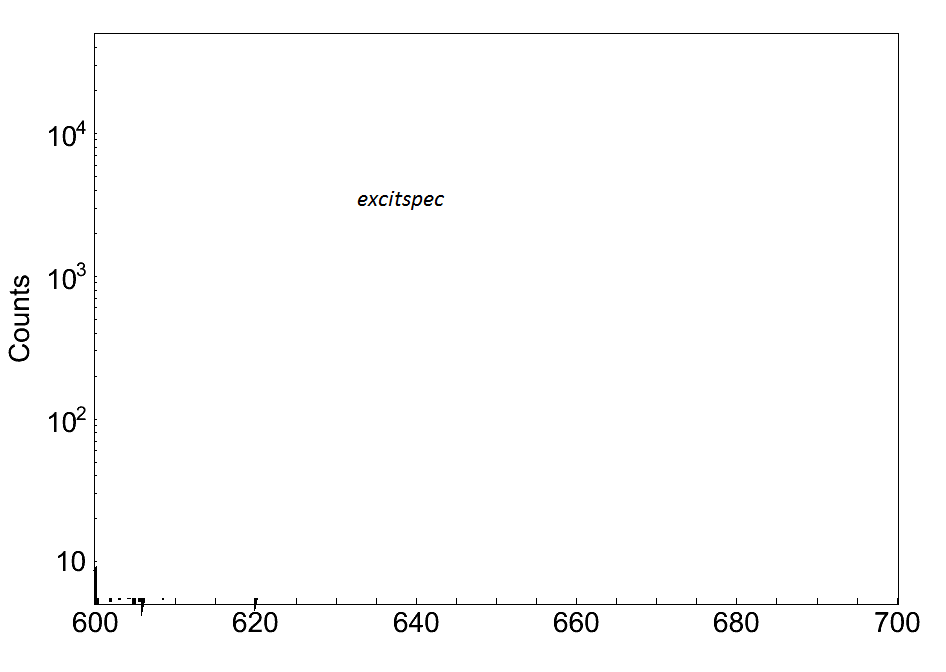
\includegraphics[width=.7\textwidth]{figures/Cr_b.png}
                \caption{Sapphire bulk emission with 562-nm excitation at 11~K (a), and excitation spectrum of the sharp 694-nm emission peak using three different laser dyes (b).  Relative heights of Coumarin and Rhodamine are not exact, as excitation rates are different between experiments.  R110 and R6G were scaled to match at their boundary for the same reason.}
\label{fig:Cr}
\end{figure}

\begin{figure} %[H]
        \centering
                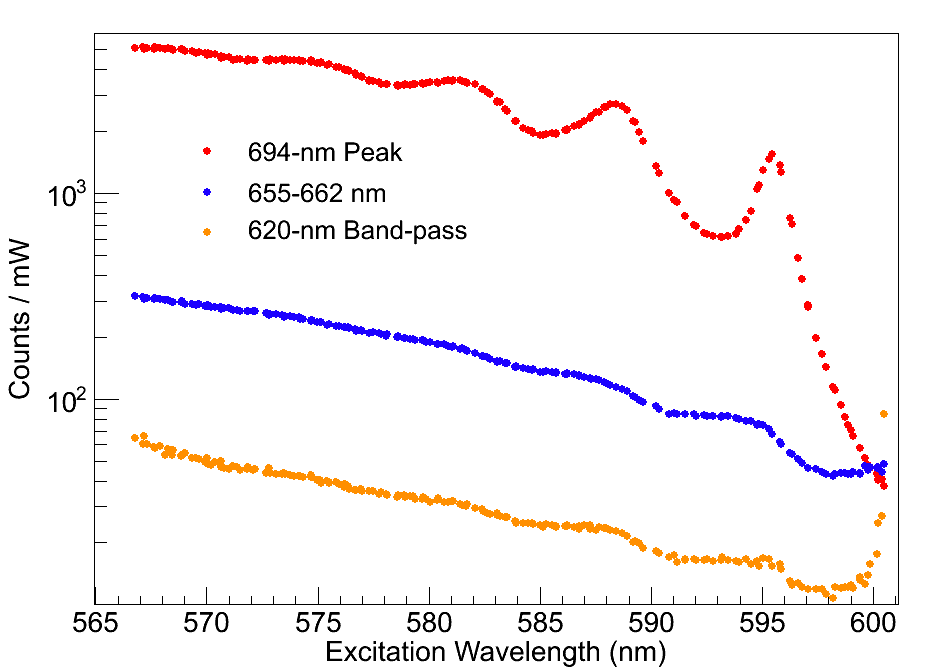
\includegraphics[width=.7\textwidth]{figures/Cr_broad.png}
                \caption{Excitation spectra for weaker sapphire bulk emissions (blue,orange) along with that of the sharp 694-nm emission (red).}
        \label{fig:CrBroad}
\end{figure}

Another source of background is fluorescence from the sapphire window.  A spectrum of this fluorescence with 562~nm excitation is shown in Fig. \ref{fig:Cr}(a).  The strong, sharp peak at 694~nm is a well-known emission of Cr\textsuperscript{3+} impurities in the sapphire bulk.  An excitation spectrum for this peak is shown in Fig. \ref{fig:Cr}(b) over the range all three dyes R6G, R110, and C480, using a sapphire window with relatively high Cr\textsuperscript{3+} content.  Multiple features observed in the excitation spectrum are consistent with the absorption spectrum of Cr\textsuperscript{3+} in sapphire at 77~K, including three sharp peaks in the blue, and a broad absorption in the green/yellow with vibrational peaks on the red tail \cite{SapphireFord,SapphireMcclure}.  In addition to the 694-nm peak, a weaker and much broader emission is observed, along with three weak peaks around the 619-nm Ba peak region, also from the sapphire bulk.  Excitation spectra for these fluorescence components are shown in Fig. \ref{fig:CrBroad} for the R6G dye range.  In this experiment, the laser was de-focused to about w = 200~$\mu$m, and the emission observed was from the surface laser spot.  As a result, there is contribution of the surface background in the spectrum; this is negligible for the prominent 694-nm peak, however its features, broad excitation with rises near 600~nm and 567~nm, can be seen in the excitation spectra of the weaker components (blue, and especially orange curves in Fig. \ref{fig:CrBroad}).  Nonetheless, observation of the same vibrational peaks as in the 694-nm peak demonstrates that the broad emission and weak peaks in the 620 band-pass (Fig. \ref{fig:Cr}(a)) are also due to Cr\textsuperscript{3+} in the sapphire.  Commercially available c-plane quality sapphire windows contain very low concentrations of Cr\textsuperscript{3+}.   from a few companies were tested, and those from Meller Optics produced the lowest sapphire bulk emission in the 620-nm band-pass region.  The choice of 570~nm for excitation of the 619-nm fluorescence peak was made by an optimization of $S$/$\sqrt{B}$, where $S$ is the 619-nm signal and the background $B$ is the broad emission in the 620 band-pass filter region (orange curve in Fig. \ref{fig:CrBroad}).  The Cr\textsuperscript{3+} emission has an inverse relationship with temperature, shown in Fig. \ref{fig:BGtempDependence}.

%with Cr\textsuperscript{3+} concentrations of around {\color{red}10 ppt} observed.

%(peaks around? May need to ask Bill about what peaks exist and at what temps ... a new idea is to just leave it vague, as ``peaks" since you're sure there are at least 2, but vauge is OK)

\section{Candidate Ba\textsuperscript{+} Lines/Blue Excitation}
\label{sec:BaPlus}

Since the fraction of neutralization of Ba\textsuperscript{+} deposited in SXe is not known to be 100\%, in this system and particularly in future tests of grabbing out of LXe, detection of single Ba\textsuperscript{+} in SXe is still of interest.  Preliminary studies of fluorescence from Ba\textsuperscript{+} deposits were performed by blue laser excitation with the C480 dye laser.

\begin{figure} %[H]
        \centering
                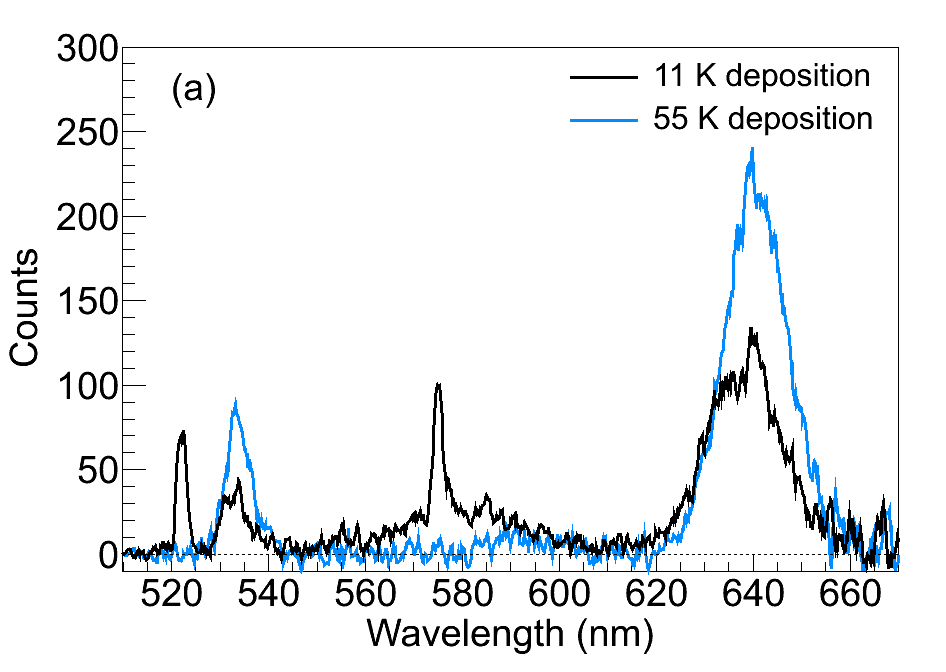
\includegraphics[width=.5\textwidth]{figures/BaHx_a.png}
                ~
                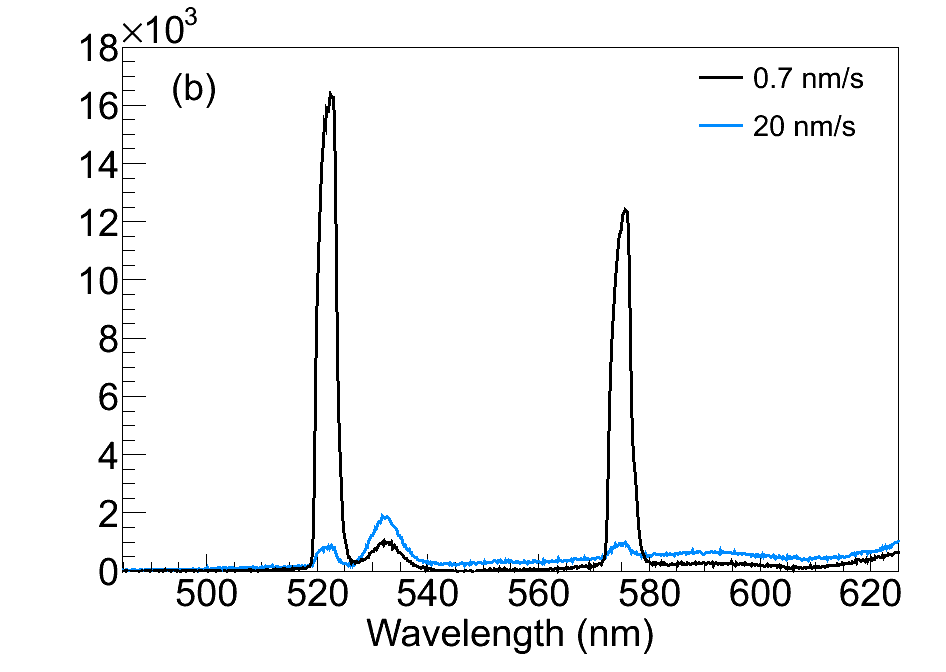
\includegraphics[width=.5\textwidth]{figures/BaHx_b.png}
                \caption{Comparison of Ba\textsuperscript{+} deposits made at (a) 55~K vs. 11~K, and (b) 20~nm/s vs. 0.7~nm/s.\cite{Mong2015}}
\label{fig:BaHx}
\end{figure}

Blue excitation of Ba\textsuperscript{+} in SXe were first explored in the thesis of Shon Cook, wherein a set of sharp emission peaks were observed at 522, 575, 637, 712, and 814~nm, in decreasing amplitude.  These peaks were attributed to emission from different vibrational states of a molecule composed of Ba and one or more H atoms \cite{Shon}.  This attribution is supported by two experiments.  Firstly, a reduction of those peaks is observed in deposits made at 50~K, well above the H$_{2}$ freezing temperature of 12~K, vs. deposits made at 11~K, as shown in Fig. \ref{fig:BaHx}(a).  Secondly, the peaks are much stronger in deposits made with lower leak rates, as shown in Fig. \ref{fig:BaHx}(b), for deposits made at 11~K.  This is explained by a higher concentration of H$_{2}$ impurities in a matrix formed with a lower leak rate.

\begin{figure} %[H]
        \centering
                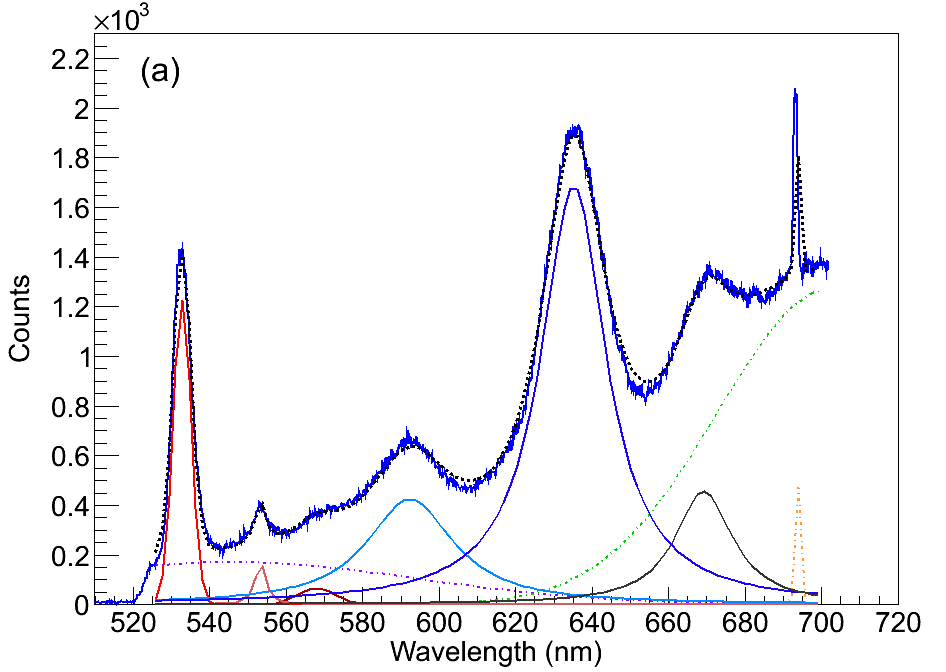
\includegraphics[width=.7\textwidth]{figures/excitspecBlue_a.png}
                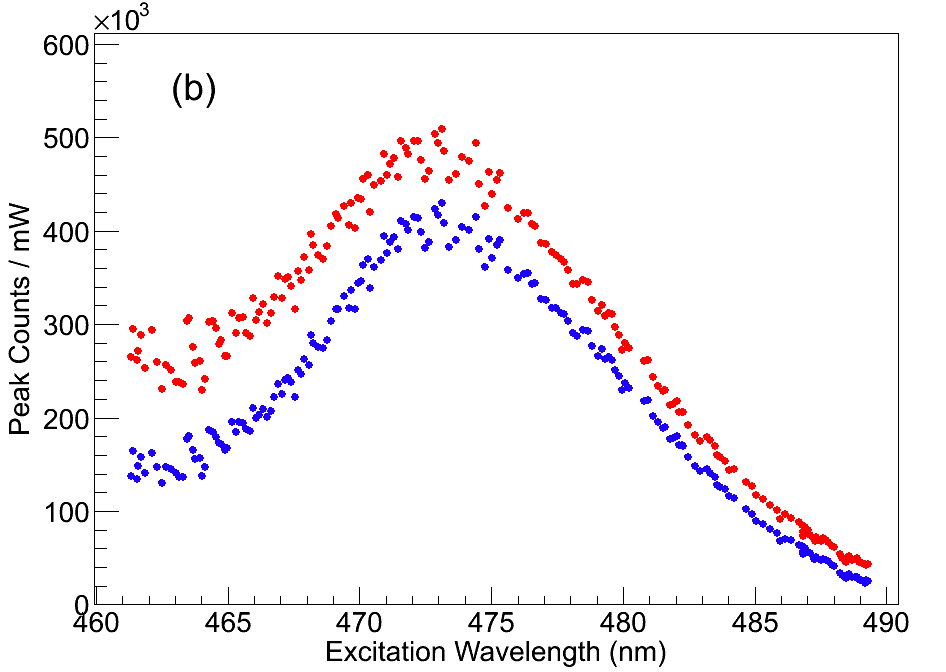
\includegraphics[width=.7\textwidth]{figures/excitspecBlue_b.png}
                \caption{(a) Multiple-component fit to example emission spectrum with 468.2-nm excitation, and (b) excitation spectra for peaks observed through C480 dye range.  In (a), the 532- and 568-nm peaks are fit with Gaussians, and the 553-, 592-, 635- and 669-nm peaks are fit with Lorentzians.}
\label{fig:excitspecBlue}
\end{figure}

In contrast to lower BaH$_{x}$ emission, several other emission peaks become prominent in deposits made at 50$\pm$5~K and observed at 11~K.  A representative spectrum with fits is shown in Fig. \ref{fig:excitspecBlue}(a), and excitation spectra from those fits over the C480 dye range are shown in Fig. \ref{fig:excitspecBlue}(b).  \emph{\color{gray}The broad blue BG ... what does its excitspec look like? is it possible it is the surface BG? ... anyway you need to mention it.}  Of particular interest are the peaks at 532~nm and 635~nm.  These peaks have identical excitation spectra, indicating that they are due to the same excitation transition.  Thus the 532- and 635-nm peaks may be due to relaxation to the ground and metastable D states, respectively, from one of the excited P states of Ba\textsuperscript{+} in SXe.  However, matrix effects would need to be responsible for the higher number of counts observed in the 635nm peak vs. the 532-nm peak, whereas the P $\rightarrow$ S transition is about 4$\times$ more likely than the P $\rightarrow$ D transition in vacuum.  The resemblance between the excitation spectra for the 592- and 669-nm peaks, as well as between the 553- and 568-nm peaks, is also interesting.  

%(a) the much slower bleaching rate than would be observed by optical pumping of Ba\textsuperscript{+} in vacuum, and (b)

%, as well as identical bleaching rates, shown in Fig. [fig 532/635 bleach]